%%%%%%%%%%%%%%%%%%%%%%%%%%%%%%%%%%%%%%%%%%%%%%%%%%%%%%%%%%%%%%%%%
% MUW Presentation
% LaTeX Template
% Version 1.0 (27/12/2016)
%
% License:
% CC BY-NC-SA 4.0 (http://creativecommons.org/licenses/by-nc-sa/3.0/)
%
% Created by:
% Nicolas Ballarini, CeMSIIS, Medical University of Vienna
% nicoballarini@gmail.com
% http://statistics.msi.meduniwien.ac.at/
%
% Customized for UAH by:
% David F. Barrero, Departamento de Automática, UAH
%%%%%%%%%%%%%%%%%%%%%%%%%%%%%%%%%%%%%%%%%%%%%%%%%%%%%%%%%%%%%%%%%

\documentclass[10pt,compress]{beamer} % Change 10pt to make fonts of a different size
\mode<presentation>

\usepackage[spanish]{babel}
\usepackage{fontspec}
\usepackage{tikz}
\usepackage{etoolbox}
\usepackage{xcolor}
\usepackage{xstring}
\usepackage{listings}

\usetheme{UAH}
\usecolortheme{UAH}
\setbeamertemplate{navigation symbols}{} 
\setbeamertemplate{caption}[numbered]

%%%%%%%%%%%%%%%%%%%%%%%%%%%%%%%%%%%%%%%%%%%%%%%%%%%%%%%%%%%%%%%%%
%% Presentation Info
\title[OOP concepts]{Object-Oriented Programming concepts}
\author{}
\institute{\asignatura}
\date{}
%%%%%%%%%%%%%%%%%%%%%%%%%%%%%%%%%%%%%%%%%%%%%%%%%%%%%%%%%%%%%%%%%


%%%%%%%%%%%%%%%%%%%%%%%%%%%%%%%%%%%%%%%%%%%%%%%%%%%%%%%%%%%%%%%%%
%% Descomentar para habilitar barra de navegación superior
\setNavigation
%%%%%%%%%%%%%%%%%%%%%%%%%%%%%%%%%%%%%%%%%%%%%%%%%%%%%%%%%%%%%%%%%

%%%%%%%%%%%%%%%%%%%%%%%%%%%%%%%%%%%%%%%%%%%%%%%%%%%%%%%%%%%%%%%%%
%% Configuración de logotipos en portada
%% Opacidad de los logotipos
\newcommand{\opacidad}{1}
%% Descomentar para habilitar logotipo en pié de página de portada
\renewcommand{\logoUno}{Images/isg.png}
%% Descomentar para habilitar logotipo en pié de página de portada
%\renewcommand{\logoDos}{Images/CCLogo.png}
%% Descomentar para habilitar logotipo en pié de página de portada
%\renewcommand{\logoTres}{Images/ALogo.png}
%% Descomentar para habilitar logotipo en pié de página de portada
%\renewcommand{\logoCuatro}{Images/ELogo.png}
%%%%%%%%%%%%%%%%%%%%%%%%%%%%%%%%%%%%%%%%%%%%%%%%%%%%%%%%%%%%%%%%%

%%%%%%%%%%%%%%%%%%%%%%%%%%%%%%%%%%%%%%%%%%%%%%%%%%%%%%%%%%%%%%%%%
%% FOOTLINE
%% Comment/Uncomment the following blocks to modify the footline
%% content in the body slides. 


%% Option A: Title and institute
\footlineA
%% Option B: Author and institute
%\footlineB
%% Option C: Title, Author and institute
%\footlineC
%%%%%%%%%%%%%%%%%%%%%%%%%%%%%%%%%%%%%%%%%%%%%%%%%%%%%%%%%%%%%%%%%

\begin{document}

%%%%%%%%%%%%%%%%%%%%%%%%%%%%%%%%%%%%%%%%%%%%%%%%%%%%%%%%%%%%%%%%%
% Use this block for a blue title slide with modified footline
{\titlepageBlue
    \begin{frame}
        \titlepage
    \end{frame}
}

\begin{frame}[plain]{}
   \begin{block}{Objective}
   \begin{itemize}
   		\item Understand the meaning of paradigm
   		\item Introduce the main OOP concepts
		\item Basic Java syntax for classes
	\end{itemize}
	\end{block}

   \begin{block}{Bibliography}
      \begin{enumerate}
          \item The Java\textsuperscript{TM} Tutorials. Oracle. \href{https://docs.oracle.com/javase/tutorial/}{(Link)}
      \end{enumerate} 
   \end{block}

   \begin{block}{Readings}
      \begin{enumerate}
          \item Intro to Object-Oriented Programming for Game Development. \href{https://gamedevelopment.tutsplus.com/tutorials/quick-tip-intro-to-object-oriented-programming-for-game-development--gamedev-1805}{(Link)}
          \item Game Architecture Day 2. \href{http://blog.nuclex-games.com/2010/01/game-architecture-day-2/}{(Link)}
      \end{enumerate} 
   \end{block}
\end{frame}

{
\disableNavigation{white}
\begin{frame}[shrink]{Table of Contents}
 \frametitle{Table of Contents}
 \tableofcontents
  % You might wish to add the option [pausesections]
\end{frame}
}

\section[Programming paradigms]{Programming paradigms}

%\begin{frame}{Object-Oriented Programming}{Programming paradigms}
%	\begin{itemize}
%		\item Any programming language has a philosophy named \alert{paradigm}
%			\begin{itemize}
%			\item Imperative, functional, logical and object-oriented (OOP) programming
%			\end{itemize}
%		\item Any paradigm can be used with any language ...
%			\begin{itemize}
%			\item ... but doing OOP with assembler may be a bit tough
%			\end{itemize}
%		\item Java is a object-oriented language
%			\begin{itemize}
%			\item It is based on objects (of course) and classes
%			\end{itemize}
 % 	\end{itemize}
%\end{frame}

%\section{Object-Oriented Programming}

%\subsection[OOP objectives]{OOP objectives}

%\begin{frame}{Object-Oriented Programming}{OOP objectives}
%	OOP encourages
%	\begin{itemize}
%	\item Modularity
%	\item Encapsulation
%	\item Re-use
%	\item \scriptsize{Debugging ease}
%	\end{itemize}
%\end{frame}

\subsection{Programming, programming language and paradigm}

\begin{frame}{Programming paradigms}{Programming, programming language and paradigm}
	\begin{block}{Programming}
		Set of techniques that allow the development of programs using a programming language
	\end{block}
	\begin{block}{Programming language}
		Set of rules and instructions based on a familiar syntax and later translated into machine language which allow the elaboration of a program to solve a problem	\end{block}
	\begin{block}{Paradigm}
		Set of rules, patterns and styles of programming that are used by programming languages
%	Conjunto de estandares, teorias y metodos para representar un modo de organizar el pensamiento. % Forma de entender la realidad. 
	\end{block}

\end{frame}

\subsection[Programming paradigms types]{Programming paradigms types}

\begin{frame}{Programming paradigms}{Programming paradigms types (I)}
	\begin{center}
	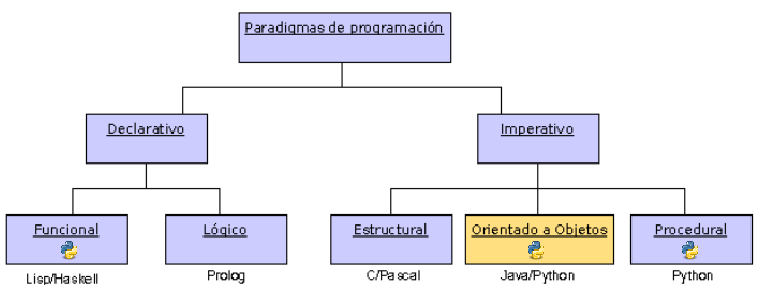
\includegraphics[scale=0.4]{figs/paradigmas}\\
	\tiny{\href{http://www.computer.org/csdl/mags/it/2011/05/mit2011050030-abs.html}{(Source)}}\\
	\end{center}
	\normalsize{Many other paradigms: Event-Driven programming, Concurrent, Reactive, Generic, etc}
\end{frame}

\subsection{Declarative programming}
\begin{frame}{Programming paradigms}{Declarative programming}
	\begin{block}{Declarative programming}
Describe \alert{what} is used to calculate through conditions, propositions, statements, etc., but does not specify how
  	\end{block}
  	\begin{itemize}
  		\item \textbf{Logic}: First order logic in order to formalize facts of the real world \textit{(Prolog)}
  		\begin{itemize}
  			\item Example: \textit{Anne's father is Raul, Raul's mother is Agnes. Who is Ana's grandmother} 
  		\end{itemize}
  		\item \textbf{Functional}: Based on the evaluation of functions (like Maths) recursively  (\textit{Lisp, Haskell, R})
  		\begin{itemize}
  			\item Example: \textit{The factorial from 0 and 1 is 1 and n is the factorial from n * factorial (n-1). What is the factorial from 3?} 
  		\end{itemize}
  	\end{itemize}
\end{frame}

\subsection{Imperative programming}

\begin{frame}{Programming paradigms}{Imperative programming}
	\begin{block}{Imperative programming}
		Describes, by a set of instructions, \alert{how} the task should be implemented  
  	\end{block}
  	\begin{itemize}
  		\item \textbf{Procedural}: Collections of subroutines related by means of invocations (\textit{C, Python})
  		\begin{itemize}
  			\item Example: \textit{The cooking process consists of 20 lines of code. When it is used, it only calls the function (1 line)} 
  		\end{itemize}
  		\item \textbf{Structural}: Nesting, loops, conditionals and subroutines. \texttt{GOTO} command is forbidden 				 \textit{(C, Pascal)}
  		\begin{itemize}
  			\item Example: \textit{Reviewing products of a shopping list and add the item X to the shopping if it is available} 
  		\end{itemize}
  	\end{itemize}
\end{frame}

\subsection{Object-Oriented Programming}

\begin{frame}{Programming paradigms}{Object-Oriented Programming}
	\begin{block}{Object-Oriented Programming}
		Evolves from imperative programming. It is based on \alert{objects} that allow express the \alert{attributes} and \alert{behavior} in a closer way to real life (\textit{Java, Python, C++, C\#})
  	\end{block}
  	\begin{itemize}
  		\item \textbf{Main characteristics}: Abstraction, encapsulation, polymorphism, inheritance, modularity, etc
        \begin{itemize}
		\item Example: \textit{A car has a set of properties (color, fuel type, model) and a functionality (speed up, shift gears, braking)} 
        \end{itemize}
  	\end{itemize}
\end{frame}

\subsection{OOP objectives}

\begin{frame}{Programming paradigms}{OOP objectives}
OOP tries to provide
\begin{itemize}
  	\item \textbf{Reusability}: Ability of software elements to serve for many applications
	\item \textbf{Modularity}: Capacity to divide a program
  	\item \textbf{Extensibility}: Ease of adapting software products to specification changes
  	\item \textbf{Usability}: Ease of using the tool
\end{itemize} 	
OOP relays on a set of abstract concepts
\end{frame}


\section[Object-Oriented Programming]{Object-Oriented Programming}

\subsection{Basic concepts}

\begin{frame}{Object-Oriented Programming}{Basic concepts (I)}
	\begin{block}{Class}
		 Generic entity that groups the \alert{properties} and \alert{functions} of an entity
  	\end{block}	
		\begin{figure}
			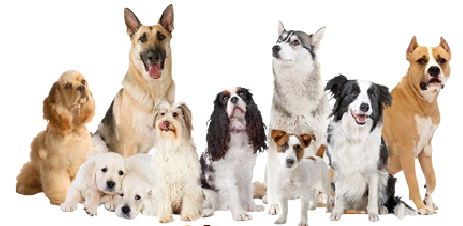
\includegraphics[scale=0.5]{figs/clase}	
		\end{figure}				
\end{frame}

\begin{frame}{Object-Oriented Programming}{Basic concepts (II)}
	\vfill\begin{block}{Atribute}
		Individual characteristics that determine the qualities of an object
  	\end{block}	
		\begin{figure}
			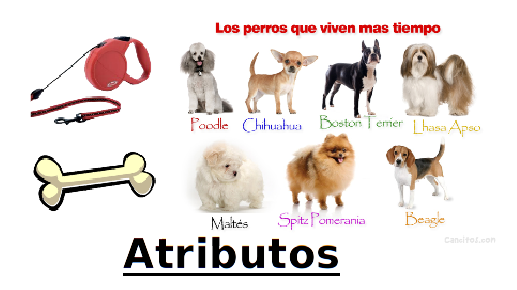
\includegraphics[scale=0.5]{figs/atributo}
		\end{figure}				
\end{frame}

\begin{frame}{Object-Oriented Programming}{Basic concepts (III)}
	\vfill\begin{block}{Method}
		 Function responsible for performing operations
  	\end{block}	
		\begin{figure}
			
\includegraphics[scale=0.5]{figs/metodo}
		\end{figure}				
\end{frame}

\begin{frame}{Object-Oriented Programming}{Basic concepts (IV)}
	\vfill\begin{block}{Object or instance}
		 Specific representation of a class, namely, a class member with their corresponding attributes
  	\end{block}	  	
		\begin{figure}
			
\includegraphics[scale=0.5]{figs/instancia}
		\end{figure}				
\end{frame}

\begin{frame}{Object-Oriented Programming}{Basic concepts (V)}
	\begin{block}{Constructor}
		 Method called when an object is created. It allows the initialization of attributes
  	\end{block}	
		\begin{figure}
			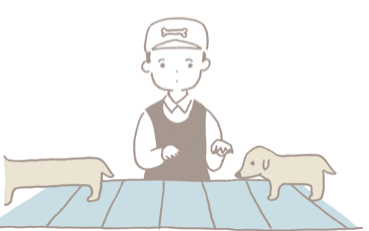
\includegraphics[scale=0.5]{figs/constructor}
		\end{figure}				
\end{frame}

\subsection{Synthesizing OOP terminology}
\begin{frame}{Object-Oriented Programming}{Synthesizing OOP terminology (I)}
%    \begin{columns}
% 	   \column{.6\textwidth}
 		  \begin{itemize}
			\item Software objects mimics physical objects % un  individuo o ejemplar de una clase 
		   	\begin{itemize}
				\item An object contains \textit{attributes} and a \textit{behaviour} % behavior u operaciones
				\item Example: A dog has a name (attribute) and may bit (behaviour)
		  	\end{itemize}
		  %	\item Objects are grouped into classes.
		  	\item A \alert{class} is a set of objects with common characteristics and behaviour
		  	\item An \alert{object} is called an \alert{instance} of a class
		  	% It can also be described as a pattern or template that is used to create objects.
			\item \textit{Members} of a class:
		    	\begin{itemize}
				\item \alert{Properties}: Data describing an object
				\item \alert{Methods}: What an object can do %Something that can be done to object. % o procedimiento perteneciente a un objeto.
					% modo en que se comunican los objetos entre síi. 
		  	    \end{itemize}
			% \item Property = Member, attribute, variable, etc.
		  \end{itemize}
 		%\column{.4\textwidth}
	  	 %	\begin{figure}[t]
		%	\begin{center}
		%	    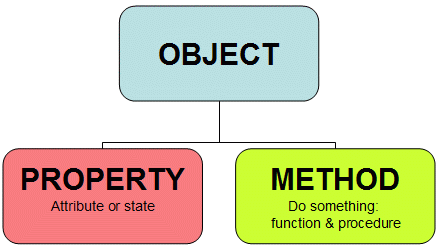
\includegraphics[width=0.97\linewidth]{figs/object2}\\
		%		\tiny{Source: http://www.teachitza.com/delphi/oop.htm}
		%	\end{center}
  	 	%	\end{figure}
%    \end{columns}
\end{frame}

\begin{frame}[plain]{Object-Oriented Programming}{Synthesizing OOP terminology (II)}
	\begin{center}
	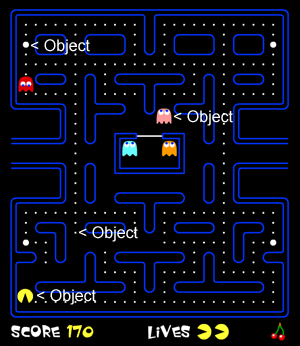
\includegraphics[width=0.6\linewidth]{figs/pacman}\\
	\smallskip
	\tiny{\href{http://blog.sklambert.com/introduction-to-oop-for-game-development/}{(Source)}}
	\end{center}
\end{frame}

\begin{frame}[plain]{Object-Oriented Programming}{Synthesizing OOP terminology (III)}
	\begin{center}
    	\centering 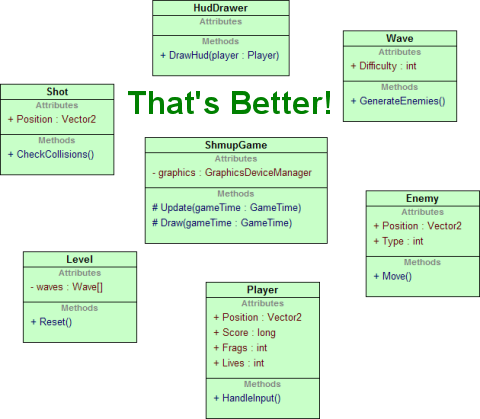
\includegraphics[width=0.8\linewidth]{figs/gameObjects}\\
		\smallskip
		\tiny{\href{http://blog.nuclex-games.com/2010/01/game-architecture-day-2/}{(Source)}}
	\end{center}
\end{frame}



%Diapositiva del Main
%\begin{frame}{Programación Orientada a Objetos(I) - Definiciones (VI)}{}
%	\begin{block}{Main}
%		 \justifying Módulo principal muy util para la realización de pruebas. Permite incluir solamente los fragmentos de código que quieran ser probados.
%  	\end{block}	
%		\vspace{1cm}
%		\centering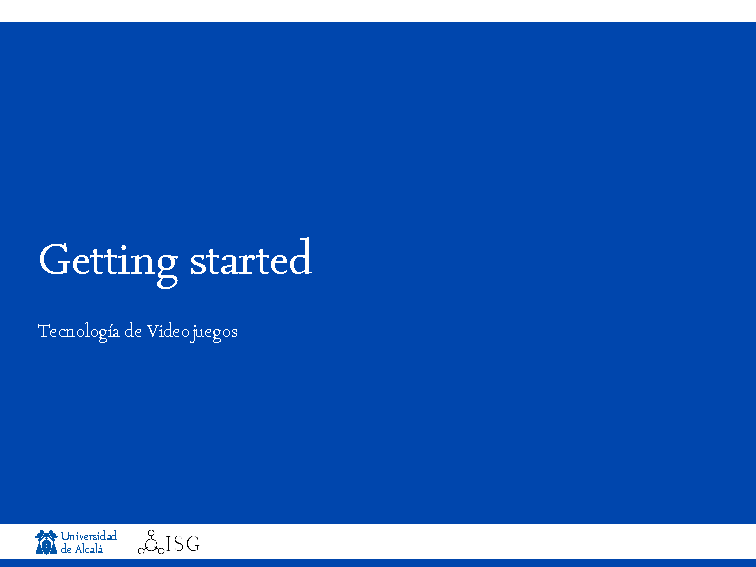
\includegraphics[scale=0.1]{figs/main}
%\end{frame}


\subsection{Inheritance}

\begin{frame}{Object-Oriented Programming}{Inheritance (II)}
\vspace{-0.2cm}
	\begin{block}{}
	Mechanism of \alert{reusing} code in OOP. Consists of generating child classes from other existing (\alert{super-class}) allowing the use and adaptation of the attributes and methods of the parent class to the child class
  	\end{block}	
\vspace{-0.2cm}
\begin{itemize}
	\item \textit{Superclass}: ``Father'' of a class
	\item \textit{Subclass}: ``Child'' of a class
	\item A subclass inherits all the attributes and methods from its superclass
	\item \textit{Class hierarchy}: A set of classes related by inheritance
\end{itemize}
\end{frame}

\begin{frame}{Object-Oriented Programming}{Inheritance (II)}
	\begin{center}
		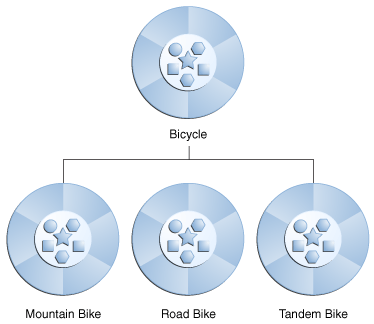
\includegraphics[width=0.5\linewidth]{figs/concepts-bikeHierarchy2}\\
	
		\tiny\href{http://docs.oracle.com/javase/tutorial/java/concepts/inheritance.html}{(Source)}
	\end{center}
\end{frame}

\begin{frame}{Object-Oriented Programming}{Inheritance (III)}
	\begin{figure}
		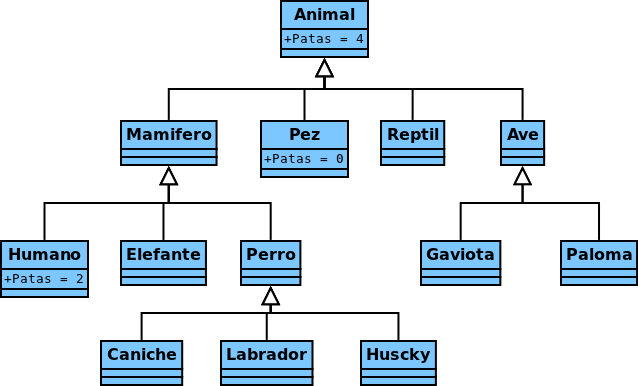
\includegraphics[scale=0.4]{figs/herencia1}\\
		\tiny{\href{http://android.scenebeta.com}{(Source)}}
	\end{figure}
\end{frame}

\begin{frame}{Object-Oriented Programming}{Inheritance (IV)}
	\centering 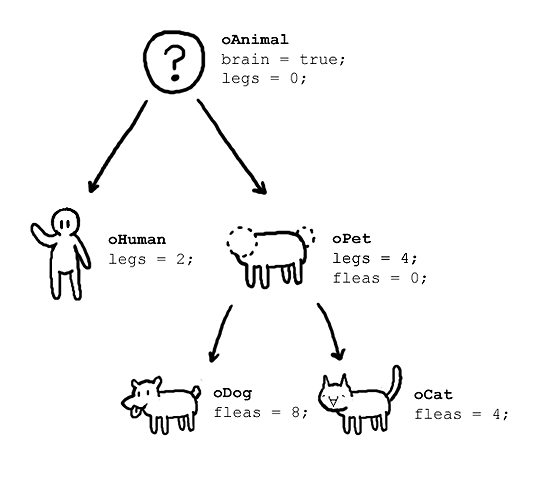
\includegraphics[width=0.7\linewidth]{figs/hierarchyGame}\\
	\bigskip
	\centering \tiny{Source: http://forums.tigsource.com/index.php?topic=3630.0}
\end{frame}


\subsection{Polymorphism}
\begin{frame}{Object-Oriented Programming}{Polymorphism (I)}
\vspace{-0.2cm}
	\begin{block}{Polymorphism}
		Invoke a method whose implementation will depend on the object that contains it
  	\end{block}	
% TIPOS DE POLIMORFISMO
%		\begin{itemize}
%			\item \justifying\textbf{Polimorfismo de sobrecarga}: mismo nombre y tipos de 						  datos en diferentes clases.
%			\item \justifying\textbf{Polimorfismo paramétrico}: mismo nombre diferentes 							  tipos de datos. 
%			\item \justifying\textbf{Polimorfismo de subtipado}: Permite invocar un método 						  de una clase especializada a partir de la clase padre.
%		\end{itemize}
	\begin{figure}
	  \vspace{-0.2cm}
		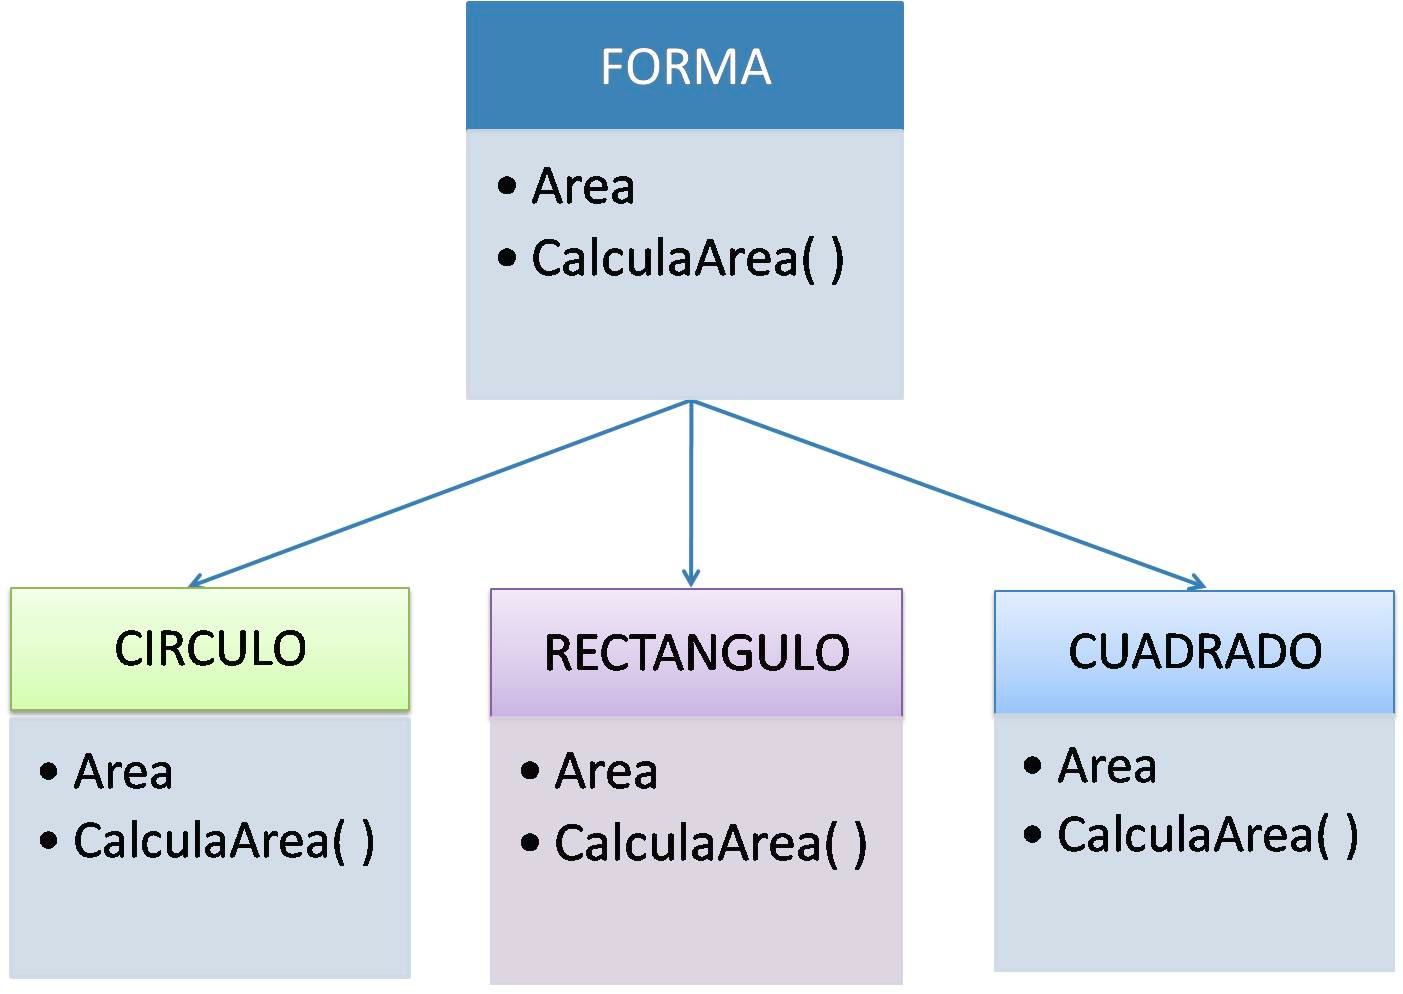
\includegraphics[width=4.6cm]{figs/polimorfismo1}\\
		\tiny{\href{http://virtual.uaeh.edu.mx}{(Source)}}
	\end{figure}
\end{frame}

\begin{frame}{Object-Oriented Programming}{Polymorphism (II)}
	\begin{figure}
		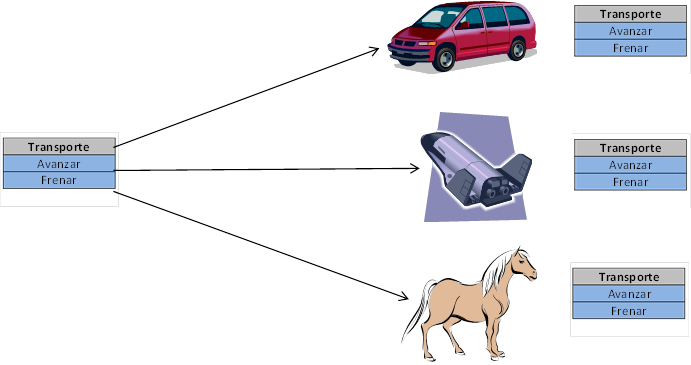
\includegraphics[scale=0.5]{figs/polimorfismo2}\\
		\tiny{\href{http://datateca.unad.edu.co}{(Source)}}
	\end{figure}
\end{frame}

\subsection{Abstraction and encapsulation}

\begin{frame}{Object-Oriented Programming}{Abstraction}
	\begin{block}{Abstraction}
		Mechanism that allows the isolation of the not relevant information to a level of knowledge
  	\end{block}	
	
	\begin{itemize}
		\item \textit{A driver does not need to know how the carburator works} 
		\item \textit{To talk on the phone does not need to know how the voice is transferred} 
		\item \textit{To use a computer do not need to know the internal composition of their materials}
		
%		\vfill\item \textit{\alert{En Python no existen de manera nativa las clases 					abstractas pero si mediante el módulo ABC \cite{PythonTeam}.}}
	\end{itemize}
\end{frame}

\begin{frame}{Object-Oriented Programming}{Encapsulation}
	\begin{block}{Encapsulation}
		Provide an access level to methods and attributes for avoiding unexpected state changes. This mechanism is used to limit the visibility of the attributes and to create methods controlling them (\texttt{set()} y \texttt{get()}).
  	\end{block}	
	
	The most common access levels are:
	
	\begin{itemize}
		\item \textbf{public}: visible for everyone
		\item \textbf{private}: visible for the creator class
		\item \textbf{protected}: visible for the creator class and its descendents
	\end{itemize}
\end{frame}

%\begin{frame}{Characteristics}{Abstraction and encapsulation (III). Example 1}
%	\begin{figure}
%		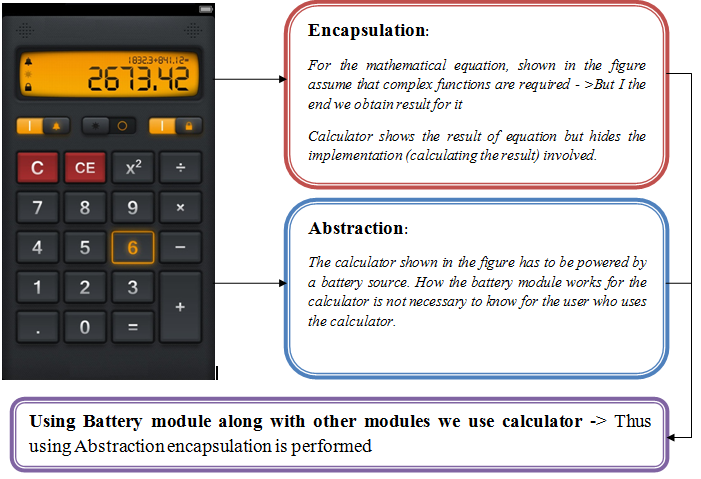
\includegraphics[scale=0.4]{figs/abstraccion1}
%		\caption{{\scriptsize Example of abstraction and encapsulation.Obtained from: \url{https://binalparekh.wordpress.com}}}
%	\end{figure}
%\end{frame}


\section{Java OOP concepts}
\subsection{Classes in Java}
\begin{frame}{Java OOP concepts}{Classes in Java (I)}
	\vspace{-0.4cm}
    \begin{columns}
 	   \column{0.8\textwidth}
			\begin{block}{Bicycle.java}
			\vspace{-0.3cm}
				\lstinputlisting[language=java, basicstyle=\ttfamily\scriptsize]{code/Bicycle.java}
			\end{block}
	\end{columns}
\end{frame}

\begin{frame}{Java OOP concepts}{Classes in Java (II)}
	\vspace{-0.4cm}
    \begin{columns}
 	   \column{.90\textwidth}
			\begin{block}{BicycleDemo.java}
			\vspace{-0.3cm}
				\lstinputlisting[language=java, basicstyle=\ttfamily\scriptsize]{code/BicycleDemo.java}
			\end{block}
	\end{columns}
\end{frame}

\subsection[Inheritance]{Inheritance in Java}

\begin{frame}{OOP concepts}{Inheritance in Java (I)}
	\vspace{-0.3cm}
    \begin{columns}
 	   \column{.90\textwidth}
			\begin{block}{BicycleDemoInheritance.java}
			\vspace{-0.2cm}
				\lstinputlisting[language=java, basicstyle=\ttfamily\scriptsize]{code/BicycleDemoInheritance.java}
			\end{block}
	\end{columns}
\end{frame}

\subsection{Interfaces}

\begin{frame}{Java OOP concepts}{Interfaces (I)}
	\textbf{Interface}: Set of methods without implementation
		\begin{itemize}
		\item Methods related to each other
		\item Expose a behaviour
		\item All methods in a interface must be implemented
		\item \textit{Imitates multiple inheritance}
		\item Interfaces can be instanciated
		\end{itemize}
\end{frame}

\begin{frame}{Java OOP concepts}{Interfaces (II)}
			\begin{block}{Bicycle.java}
			\vspace{-0.2cm}
				\lstinputlisting[language=java, basicstyle=\ttfamily\scriptsize]{code/BicycleInterface.java}
			\end{block}
			\begin{block}{ACMEBicycle.java}
			\vspace{-0.2cm}
				\lstinputlisting[language=java, basicstyle=\ttfamily\scriptsize]{code/ACMEBicycle.java}
			\end{block}
\end{frame}

\subsection{Packages}

\begin{frame}{Java OOP concepts}{Packages (I)}
	\begin{itemize}
	\item A typical Java project might content thousands of classes
		\begin{itemize}
		\item Some kind of classes organization is needed
		\end{itemize}
	\item \textbf{Package}: A collection of related classes
		\begin{itemize}
		\item Packages are ``folders'' of classes
		\item ... there is a direct mapping package-folder, indeed
		\item Technically speaking, packages separate namespaces
		\item Packages are defined using \alert{package} in the begining of a class
		\end{itemize}
	\item Packages must be declared to be used within a class
		\begin{itemize}
		\item Reserved word \alert{import}
		\end{itemize}
	\end{itemize}
	\centering 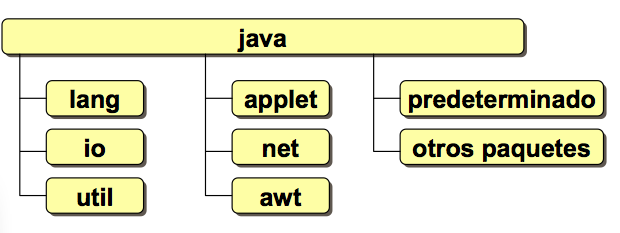
\includegraphics[width=0.5\linewidth]{figs/paquetesJava.png}\\
\end{frame}

\begin{frame}{Java OOP concepts}{Packages (II)}
	\vspace{-0.2cm}
	\begin{block}{bicycles/ACMEBicycle.java}
	\vspace{-0.2cm}
		\lstinputlisting[language=java, basicstyle=\ttfamily\scriptsize]{code/BicyclePackages.java}
		\vspace{-0.2cm}
	\end{block}
	\begin{block}{demo/BicycleDemo.java}
	\vspace{-0.2cm}
		\lstinputlisting[language=java, basicstyle=\ttfamily\scriptsize]{code/BicycleMainPackages.java}
		\vspace{-0.2cm}
	\end{block}
\end{frame}

\begin{frame}{Java OOP concepts}{Packages (III)}
	Compile with\\ 
	\begin{itemize}
	\item \texttt{javac bicycles/Bicycle}\\
	\item \texttt{javac demo/BicycleDemo}\\
	\end{itemize}
	Execute with\\
	\begin{itemize}
	\item \texttt{java demo.BicycleDemo}
	\end{itemize}
	Packages imported by default
		\begin{itemize}
		\item Package \texttt{java.lang}
		\item Same package
		\end{itemize}
		\alert{Watch out the CLASSPATH!}
		\begin{itemize}
		\item CLASSPATH: Environment variable, Java version of PATH
		\item It stores the packages (and classes) locations
		\end{itemize}
\end{frame}

\subsection{Javadoc}
\begin{frame}{Java OOP concepts}{Javadoc}
	\begin{itemize}
	\item Javadoc generates documentation from the source code
	\item Comments begining with \texttt{/**} are Javadoc comments
		\begin{itemize}
		\item They are included in the Javadoc documentation
		\end{itemize}
	\item Getting used to handle Javadoc is critical!
		\begin{itemize}
		\item Reference API documentation in any Java library is in Javadoc format
		\item Try to use it in your code
		\end{itemize}
	\end{itemize}
\end{frame}

\section{Exercises}
\subsection{Exercise 1: Asteroids}
	\begin{frame}{Exercise 1: Asteroids}
	\vspace{-0.3cm}
    \begin{columns}
 	   \column{.6\textwidth}
		\centering 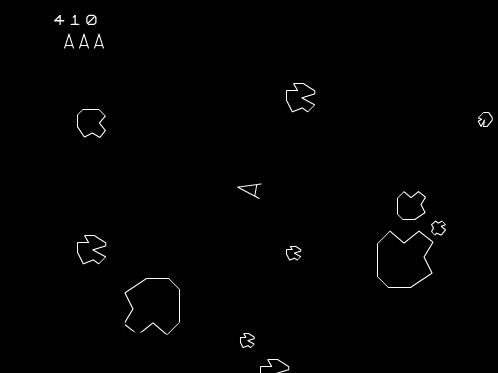
\includegraphics[width=\linewidth]{figs/asteroids.png}\\
		\tiny{\href{http://gamedevelopment.tutsplus.com/tutorials/quick-tip-intro-to-object-oriented-programming-for-game-development--gamedev-1805}{(Source)}}
		\column{.4\textwidth}
	\begin{enumerate}
	\item Identify the classes in the Asteroids videogame
	\item Identify attributes contained in the previous classes
	\item Identify methods contained in the previous classes
	\end{enumerate}
	\end{columns}
\end{frame}

\subsection{Exercise 2: Tetris}
	\begin{frame}{Exercise 2: Tetris}
    \begin{columns}
 	   \column{.4\textwidth}
		\centering 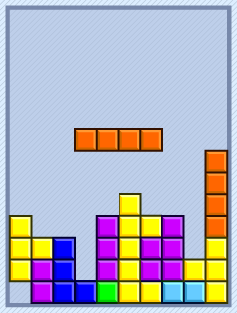
\includegraphics[width=\linewidth]{figs/tetris.png}\\
		\tiny{\href{http://gamedevelopment.tutsplus.com/tutorials/quick-tip-intro-to-object-oriented-programming-for-game-development--gamedev-1805}{(Source)}}
		\column{.4\textwidth}
	\begin{enumerate}
	\item Identify the classes in the Tetris videogame
	\item Identify attributes contained in the previous classes
	\item Identify methods contained in the previous classes
	\end{enumerate}
	\end{columns}
\end{frame}

\subsection{Exercise 3: Pac-Man}
	\begin{frame}{Exercise 3: Pac-Man}
    \begin{columns}
 	   \column{.5\textwidth}
		\centering 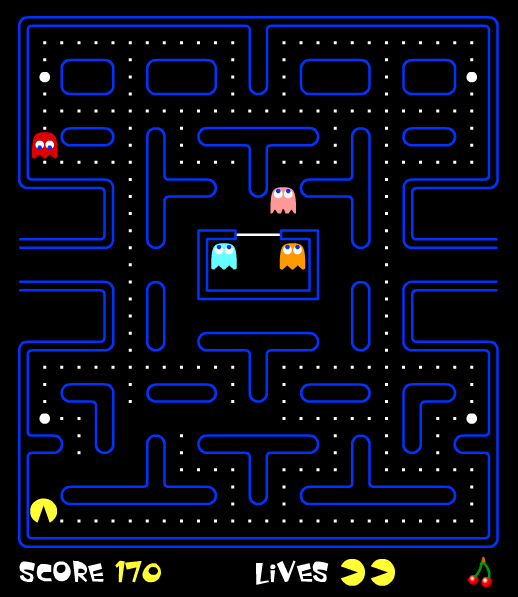
\includegraphics[width=\linewidth]{figs/pacman2.png}\\
		\tiny{\href{http://gamedevelopment.tutsplus.com/tutorials/quick-tip-intro-to-object-oriented-programming-for-game-development--gamedev-1805}{(Source)}}
		\column{.5\textwidth}
	\begin{enumerate}
	\item Identify the classes in the Pac-Man videogame
	\item Identify attributes contained in the previous classes
	\item Identify methods contained in the previous classes
	\end{enumerate}
	\end{columns}
\end{frame}




\end{document}
